\documentclass[12pt,a4paper]{article}

% 导入必要的宏包
\usepackage[UTF8]{ctex}
\usepackage{geometry}
\usepackage{amsmath}
\usepackage{amsfonts}
\usepackage{amssymb}
\usepackage{graphicx}
\usepackage{enumitem}
\usepackage{xcolor}
\usepackage{tikz}
\usepackage{float}
\usepackage{hyperref}
\usepackage{multicol}
\usepackage{longtable}
\usepackage{array}
\usepackage{tabularx}
\usepackage{listings}

% 代码高亮设置
\lstset{
    basicstyle=\ttfamily\small,
    keywordstyle=\color{blue},
    commentstyle=\color{green!70!black},
    stringstyle=\color{red},
    breaklines=true,
    numbers=left,
    numberstyle=\tiny\color{gray},
}

% 页面设置
\geometry{left=2.5cm,right=2.5cm,top=2.5cm,bottom=2.5cm}

% 标题页设置
\title{\textbf{2015年数据结构题库} \\ \large 单项选择题与综合应用题详解}
\author{}
\date{}

% 定义题型环境
\newenvironment{choicequestion}[1][]{%
    \vspace{0.5cm}
    \noindent\textbf{[#1]}
    \vspace{0.2cm}
}{}

\newenvironment{answersection}{%
    \vspace{0.2cm}
    \noindent\textbf{[参考答案]}\\
    \vspace{0.1cm}
}{}

\newenvironment{analysissection}{%
    \vspace{0.2cm}
    \noindent\textbf{[答案解析]}\\
    \vspace{0.1cm}
}{}

% 定义题号计数器
\newcounter{questioncounter}

% 定义题号计数器
\newcounter{questioncounter}

% 问题格式化命令
\newcommand{\question}[2]{%
    \stepcounter{questioncounter}%
    \noindent\textbf{\thequestioncounter} #1%
}

% 选择题选项格式
\newcommand{\choices}[4]{%
    \begin{multicols}
    \noindent \textbf{A.} #1 \par
    \noindent \textbf{B.} #2 \par
    \noindent \textbf{C.} #3 \par
    \noindent \textbf{D.} #4 \par
    \end{multicols}%
}

% 开始文档
\begin{document}

\maketitle

\section{单项选择题}

\begin{choicequestion}[单选题]
\question{已知程序如下：\newline
\begin{lstlisting}[language=C]
int S(int n)  
{ return (n <= 0)?0:S(n-1)+n;}  
void main()  
{ cout << S(1);} 
\end{lstlisting}\newline
程序运行时使用栈来保存调用过程的信息，自栈底到栈顶保存的信息依次对应的是}{}

\choices{main() $\rightarrow$ S(1) $\rightarrow$ S(0)}{S(0) $\rightarrow$ S(1) $\rightarrow$ main()}{main() $\rightarrow$ S(0) $\rightarrow$ S(1)}{S(1) $\rightarrow$ S(0) $\rightarrow$ main()}

\begin{answersection}
A. main() $\rightarrow$ S(1) $\rightarrow$ S(0)
\end{answersection}

\begin{analysissection}
程序执行时，main()首先调用S(1)。S(1)因n=1>0，继续递归调用S(0)。S(0)满足n<=0，返回0。函数调用遵循后进先出原则，调用栈从栈底到栈顶依次为：main() $\rightarrow$ S(1) $\rightarrow$ S(0)。
\end{analysissection}
\end{choicequestion}

\begin{choicequestion}[单选题]
\question{先序序列为a,b,c,d的不同二叉树的个数是}{}

\choices{13}{14}{15}{16}

\begin{answersection}
B. 14
\end{answersection}

\begin{analysissection}
先序序列固定了根结点a及各子树结点集合，但未确定左右子树划分。具有n个结点的不同二叉树个数为第n个卡塔兰数。对于n=4，第4个卡塔兰数$C_4=\frac{1}{5}\binom{8}{4}=14$。
\end{analysissection}
\end{choicequestion}

\begin{choicequestion}[单选题]
\question{下列选项给出的是从根分别到达两个叶结点路径上的权值序列，能属于同一棵哈夫曼树的是}{}

\choices{24, 10, 5 和 24, 10, 7}{24, 10, 5 和 24, 12, 7}{24, 10, 10 和 24, 14, 11}{24, 10, 5 和 24, 14, 6}

\begin{answersection}
A. 24, 10, 5 和 24, 10, 7
\end{answersection}

\begin{analysissection}
哈夫曼树中，从根到不同叶结点的路径在分叉前权值序列完全相同。选项A中两条路径前两个权值（24,10）相同，随后分叉，符合哈夫曼树结构特征。其他选项在分叉前权值存在差异，不可能属于同一棵哈夫曼树。
\end{analysissection}
\end{choicequestion}

\begin{choicequestion}[单选题]
\question{现有一棵无重复关键字的平衡二叉树（AVL 树），对其进行中序遍历可得到一个降序序列。下列关于该平衡二叉树的叙述中，正确的是}{}

\choices{根结点的度一定为 2}{树中最小元素一定是叶结点}{最后插入的元素一定是叶结点}{树中最大元素一定是无左子树}

\begin{answersection}
D. 树中最大元素一定是无左子树
\end{answersection}

\begin{analysissection}
中序遍历得到降序序列，表明该AVL树满足“左子树结点值均大于根结点值，右子树结点值均小于根结点值”（与常规BST相反）。在这样的树中，最大元素必然位于最左侧路径的末端，因此其一定无左子树。
\end{analysissection}
\end{choicequestion}

\begin{choicequestion}[单选题]
\question{设有向图 $\mathrm{G} = (\mathrm{V}, \mathrm{E})$ ，顶点集 $\mathrm{V} = \{\mathrm{v}_0, \mathrm{v}_1, \mathrm{v}_2, \mathrm{v}_3\}$ ，边集 $\mathrm{E} = \{<\mathrm{v}_0, \mathrm{v}_1>, <\mathrm{v}_0, \mathrm{v}_2>, <\mathrm{v}_0, \mathrm{v}_3>, <\mathrm{v}_1, \mathrm{v}_3>\}$ 。若从顶点 $\mathrm{v}_0$ 开始对图进行深度优先遍历，则可能得到的不同遍历序列个数是}{}

\choices{2}{3}{4}{5}

\begin{answersection}
C. 4
\end{answersection}

\begin{analysissection}
从$\mathrm{v}_0$出发，其邻接点为$\mathrm{v}_1,\mathrm{v}_2,\mathrm{v}_3$，可按不同顺序访问。$\mathrm{v}_1$还有指向$\mathrm{v}_3$的边。可能的DFS序列包括：v0-v1-v3-v2、v0-v2-v1-v3、v0-v2-v3-v1、v0-v3-v1-v2等，共4种。
\end{analysissection}
\end{choicequestion}

\begin{choicequestion}[单选题]
\question{求下面带权图的最小（代价）生成树时，可能是克鲁斯卡（Kruskal）算法第2次选中但不是普里姆（Prim）算法（从 $\mathrm{V}_4$ 开始）第2次选中的边是}{}

\begin{figure}[H]
\centering
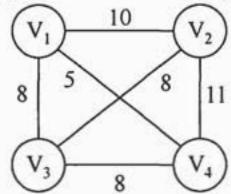
\includegraphics[width=0.3\textwidth]{images/97f00253ce52f55e799a2dae98c9137a24e15bb433588379c388e61acda7e346.jpg}
\end{figure}

\choices{$(\mathrm{V}_{1}, \mathrm{V}_{3})$}{$\left(\mathrm{V}_{1}, \mathrm{V}_{4}\right)$}{$\left(\mathrm{V}_{2}, \mathrm{V}_{3}\right)$}{$\left(\mathrm{V}_{3}, \mathrm{V}_{4}\right)$}

\begin{answersection}
B. $\left(\mathrm{V}_{1}, \mathrm{V}_{4}\right)$
\end{answersection}

\begin{analysissection}
Kruskal算法按权值从小到大依次选择不构成回路的边。Prim算法从指定顶点$\mathrm{V}_4$开始，逐步选择与已选集合相连的最小权值边。根据图中边权值关系，$(\mathrm{V}_1,\mathrm{V}_4)$可能在Kruskal第2次被选中，但在Prim从$\mathrm{V}_4$开始时并非第2次选中的边。
\end{analysissection}
\end{choicequestion}

\begin{choicequestion}[单选题]
\question{下列选项中，不能构成折半查找中关键字比较序列的是}{}

\choices{500, 200, 450, 180}{450, 200, 180}{180, 500, 200, 450}{180, 200, 500, 450}

\begin{answersection}
A. 500, 200, 450, 180
\end{answersection}

\begin{analysissection}
折半查找中，若某次比较后向左子表查找，则后续所有比较的关键字均应小于当前关键字；向右子表查找则均应大于当前关键字。选项A中500→200（向左）后出现450>200，存在矛盾，不可能构成合法比较序列。
\end{analysissection}
\end{choicequestion}

\begin{choicequestion}[单选题]
\question{已知字符串 S 为 "abaabaabacacaabaabcc", 模式串 t 为 "abaabc"。采用 KMP 算法进行匹配, 第一次出现 "失配" (s[i] ≠ t[j]) 时, i = j = 5 , 下次开始匹配时, i 和 j 的值分别是}{}

\choices{i = 1, j = 0}{i = 5, j = 0}{i = 5, j = 2}{i = 6, j = 2}

\begin{answersection}
C. i = 5, j = 2
\end{answersection}

\begin{analysissection}
模式串t="abaabc"的next数组为[-1,0,0,1,1,2]。当i=j=5失配时，按照KMP规则，主串指针i保持不变，模式串指针j回退至next[5]=2的位置。因此下次匹配时i=5，j=2。
\end{analysissection}
\end{choicequestion}

\begin{choicequestion}[单选题]
\question{下列排序算法中，元素的移动次数与关键字的初始排列次序无关的是}{}

\choices{直接插入排序}{起泡排序}{基数排序}{快速排序}

\begin{answersection}
C. 基数排序
\end{answersection}

\begin{analysissection}
基数排序通过按位分配和收集，元素的移动次数仅取决于元素个数和基数，与初始排列顺序无关。其他三种排序算法的移动次数均与初始顺序密切相关。
\end{analysissection}
\end{choicequestion}

\begin{choicequestion}[单选题]
\question{已知小根堆为8,15,10,21,34,16,12，删除关键字8之后需重建堆，在此过程中，关键字之间的比较次数是}{}

\choices{1}{2}{3}{4}

\begin{answersection}
C. 3
\end{answersection}

\begin{analysissection}
删除堆顶8后，将最后一个元素12置于堆顶，然后进行向下调整。12依次与左右孩子比较（涉及10、16、12等），共发生3次有效关键字比较。
\end{analysissection}
\end{choicequestion}

\begin{choicequestion}[单选题]
\question{希尔排序的组内排序采用的是}{}

\choices{直接插入排序}{折半插入排序}{快速排序}{归并排序}

\begin{answersection}
A. 直接插入排序
\end{answersection}

\begin{analysissection}
希尔排序的核心是将数组按增量划分为多个子序列，对每个子序列分别采用直接插入排序，随后逐步减小增量，直至增量为1。
\end{analysissection}
\end{choicequestion}

\section{综合应用题}

\begin{choicequestion}[问答题]
\question{(15分)用单链表保存 $m$ 个整数，结点的结构为[data][link]，且|data| $\leqslant n(n$ 为正整数）。现要求设计一个时间复杂度尽可能高效的算法，对于链表中 data 的绝对值相等的结点，仅保留第一次出现的结点而删除其余绝对值相等的结点。要求：\newline
1）给出算法的基本设计思想。  \newline
2）使用 C 或 $\mathrm{C}++$ 语言, 给出单链表结点的数据类型定义。  \newline
3）根据设计思想, 采用 C 或 $\mathrm{C}++$ 语言描述算法, 关键之处给出注释。  \newline
4）说明你所设计算法的时间复杂度和空间复杂度。}{}

\begin{answersection}
1) 算法的基本设计思想：使用辅助数组（大小为n+1）标记绝对值是否已出现。遍历链表，对每个结点的绝对值进行检查：若已标记，则删除该结点；否则标记并保留。
\end{answersection}

\begin{analysissection}
2) 单链表结点数据类型定义：
\begin{lstlisting}[language=C]
typedef struct Node {
    int data;
    struct Node *link;
} Node, *LinkList;
\end{lstlisting}

3) 算法实现（C语言）：
\begin{lstlisting}[language=C]
LinkList removeDuplicateAbs(LinkList head, int n) {
    if (head == NULL) return NULL;
    bool *visited = (bool *)calloc(n + 1, sizeof(bool));  // 标记数组
    Node *prev = NULL, *curr = head;
    while (curr != NULL) {
        int absVal = abs(curr->data);
        if (visited[absVal]) {  // 已出现，删除当前结点
            Node *temp = curr;
            if (prev != NULL) {
                prev->link = curr->link;
            } else {
                head = curr->link;
            }
            curr = curr->link;
            free(temp);
        } else {
            visited[absVal] = true;
            prev = curr;
            curr = curr->link;
        }
    }
    free(visited);
    return head;
}
\end{lstlisting}

4) 时间复杂度：$O(m)$（单次遍历链表）。\\
空间复杂度：$O(n)$（辅助标记数组）。
\end{analysissection}
\end{choicequestion}

\begin{choicequestion}[问答题]
\question{(8分)已知含有5个顶点的图G如下图所示。\newline

\begin{figure}[H]
\centering
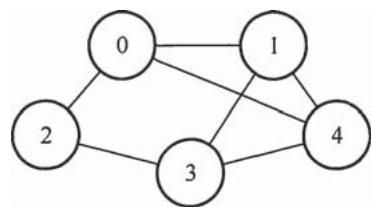
\includegraphics[width=0.3\textwidth]{images/5effb22909a8f9f41fae71fa496d27eb42d3d6f98a36725ea6d1691e02daf6c9.jpg}
\end{figure}\newline

请回答下列问题：\newline
1）写出图G的邻接矩阵 $A$ （行、列下标从0开始）。  \newline
2）求 $A^2$ ，矩阵 $A^2$ 中位于0行3列元素值的含义是什么？  \newline
3）若已知具有 $n$ （ $n \geqslant 2$ ）个顶点的图的邻接矩阵为 $B$ ，则 $B^{m}$ （ $2 \leqslant m \leqslant n$ ）中非零元素的含义是什么？}{}

\begin{answersection}
1) 图G的邻接矩阵$A$：
\[
A = \begin{bmatrix}
0 & 1 & 0 & 1 & 1 \\
1 & 0 & 1 & 1 & 0 \\
0 & 1 & 0 & 0 & 1 \\
1 & 1 & 0 & 0 & 1 \\
1 & 0 & 1 & 1 & 0
\end{bmatrix}
\]

2) $A^2$ 中0行3列元素值为从顶点0到顶点3长度为2的路径条数。

3) $B^m[i][j] \neq 0$ 表示从顶点$i$到顶点$j$存在长度为$m$的路径。
\end{answersection}

\begin{analysissection}
邻接矩阵的$m$次幂$A^m[i][j]$的数值表示从顶点$i$到顶点$j$长度恰好为$m$的路径条数。
\end{analysissection}
\end{choicequestion}

\end{document}